\section{Example: Effective Undulator Source} \label{ex14}

Since the synchrotron radiation of an undulator is
\underline{coherently} emitted from
the whole trajectory through the device, an effective source can be
defined by propagating back the field distributions calculated in a pinhole
down-stream of the device. This can be done with \W by setting

\cboxs{IPHASE=1}

To get in addition the Wigner-distributions of the source set e.g.

\cboxs{IWIGNER=-1}

The parameters for the source plane and the Wigner-distributions are defined in the namelist
\scap{\$PHASEN}. Please, have a look.

We enter in the shell:

\cboxs{\senv \grau \\
python3 ../python/wave\_example\_14.py\\
cp \$WAVE/input/wave\_example\_14.in wave.in\\ }

\W writes in this example a file
\gti{wigner.wav}\bsp, which contains the Wigner-distribution.

Of course, the set-up can and plotting can be done within the GUI
\WSH\bsp.
The radiaton cone in the pinhole down-stream of the undulator is shown
in Fig. \ref{ex14fig1}

\begin{figure}[ht]
    \centering
    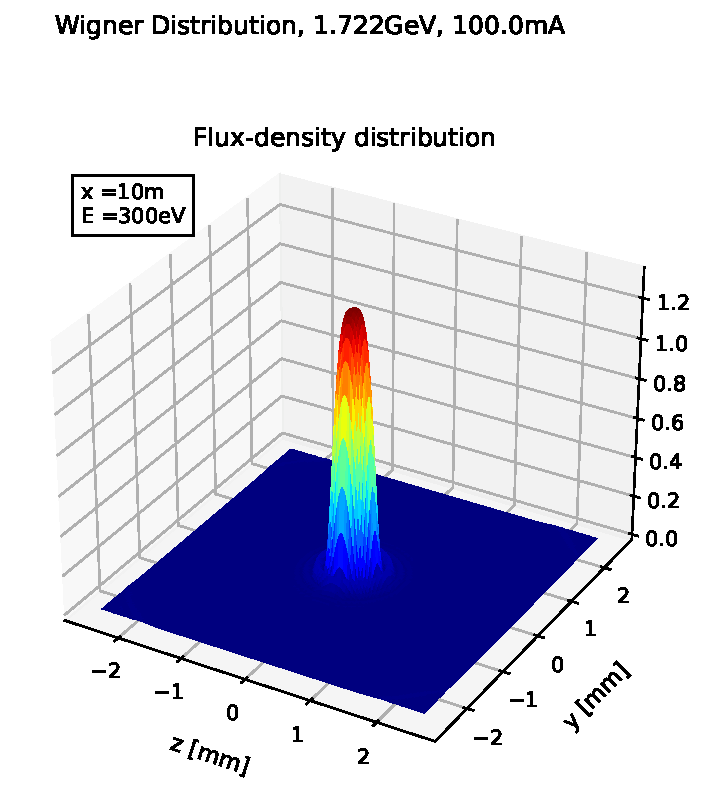
\includegraphics[width=0.55\textwidth]{pics/pin_dist.pdf}
    \caption{Radiation cone of the undulator}
    \label{ex14fig1}
\end{figure}

The fields of this cone a propagated back to the center of the
undulator. Fig. \ref{ex14fig2} shows the real part of the horizontal field.

\begin{figure}[ht]
    \centering
    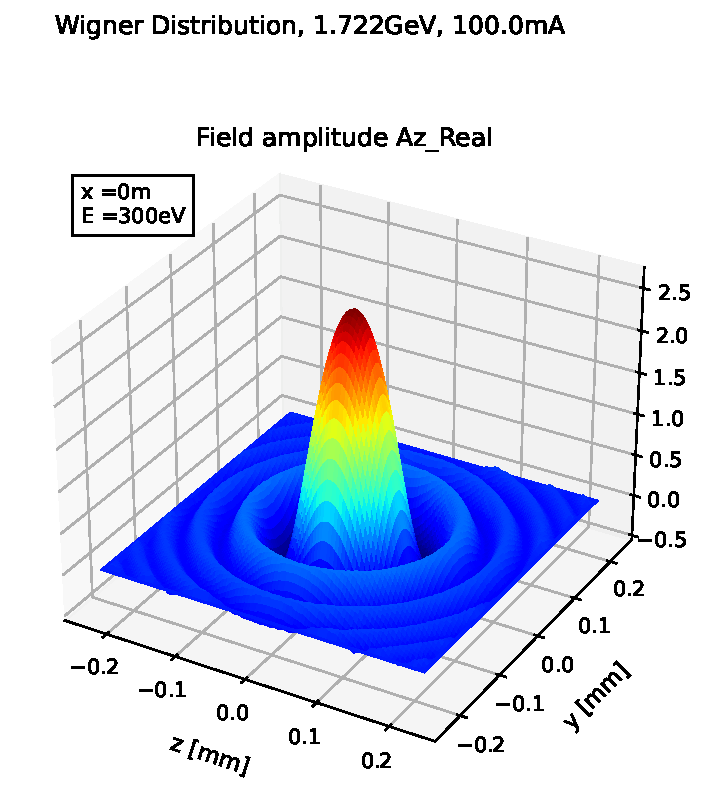
\includegraphics[width=0.55\textwidth]{pics/source_dist.pdf}
    \caption{Radiation cone of the undulator}
    \label{ex14fig2}
\end{figure}

From the back-propagated field, the Wigner-distrubtion are calculated.
Fig. \ref{ex14fig3} shows the distribution $W_{zz}$ of the horizontal
field in the $z-\Theta_z$ - plane.

\begin{figure}[ht]
    \centering
    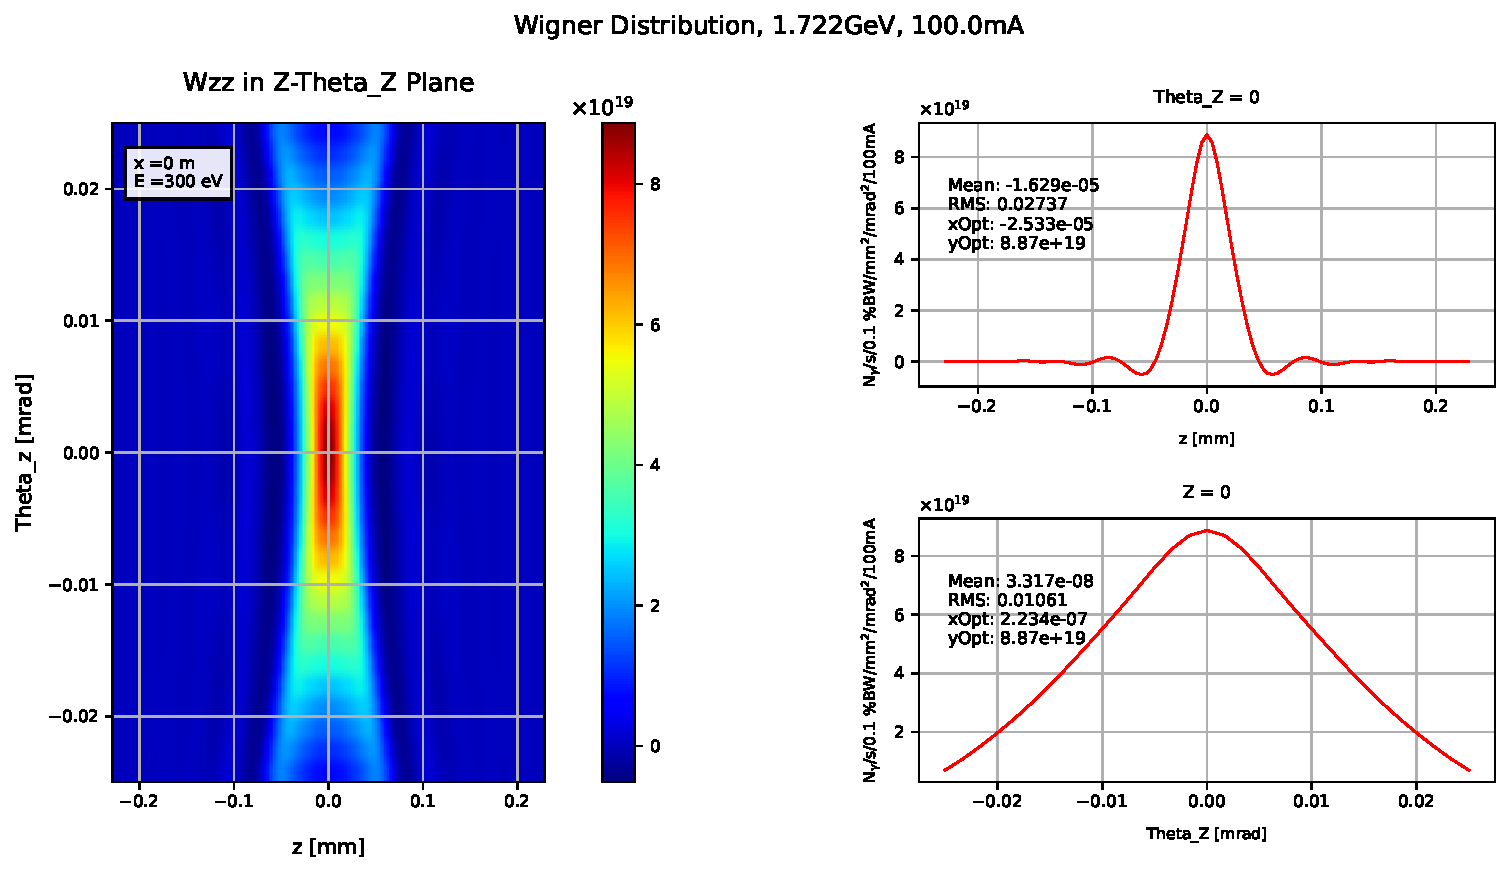
\includegraphics[width=0.75\textwidth]{pics/wigner_dist.pdf}
    \caption{Wigner-distribution $W_{zz}$ in the $z-\Theta_z$ - plane.}
    \label{ex14fig3}
\end{figure}

To include the energy-spread of the electron beam, one must set
\scap{ESPREAD} and
\scap{NWIGEFOLD}, e.g.

\cboxs{NWIGEFOLD=15}

This triggers 15 \W- runs with beam energies distributed according to
\scap{ESPREAD} and calculates the weighted integral of the
contributions and writes the results to a file named \gti{wigner.wef}.
This can be rather time consuming. The beam emittance
can be taken into account by folding the results accordingly. This is
not yet implemented in \W, but can be performed by the user on base of
the data in \gti{wigner.wef}\bsp. This file is read by \WSH, so you can
see the variables of the file in the n-tuple \gti{nwef}\bsp.

